\begin{figure}
  \centering
  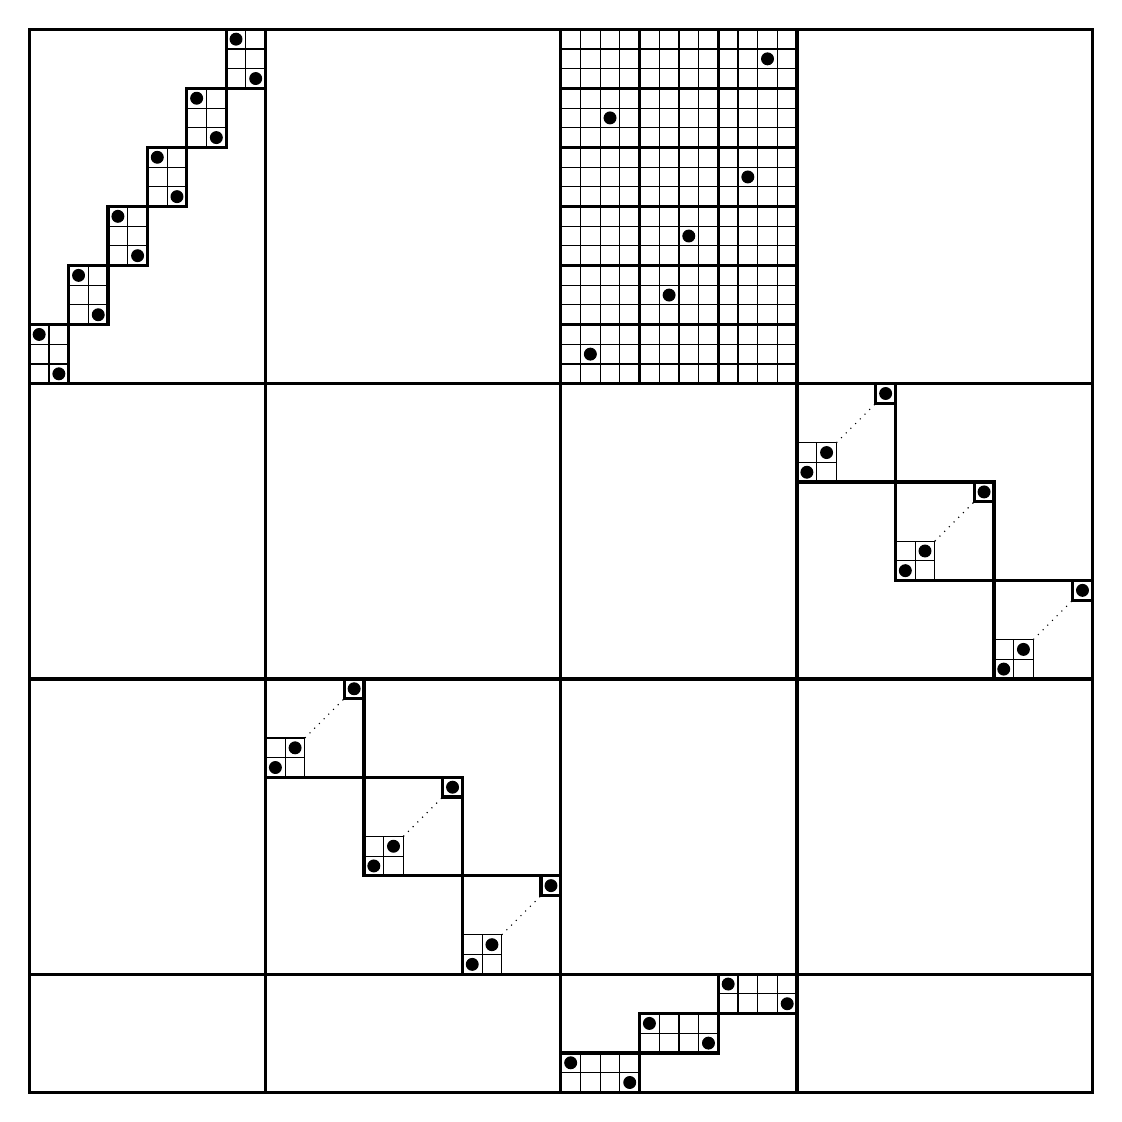
\begin{tikzpicture}
    [
      scale=.25,
    ]
    % grid
    \draw [step=1.0, black, very thick] (0,0) rectangle (54,54);
    \draw [step=1.0, black, very thick] (12,0) -- (12,54);
    \draw [step=1.0, black, very thick] (27,0) -- (27,54);
    \draw [step=1.0, black, very thick] (39,0) -- (39,54);
    \draw [step=1.0, black, very thick] (0,6) -- (54,6);
    \draw [step=1.0, black, very thick] (0,21) -- (54,21);
    \draw [step=1.0, black, very thick] (0,36) -- (54,36);

    % vertices
    \def\y{36}
    \foreach \i in {1,2,...,6} {
      \draw [step=1.0, black] (2*\i - 2, \y + 3*\i - 3) grid (2*\i, \y + 3*\i);
      \draw [black, very thick] (2*\i - 2, \y + 3*\i - 3) rectangle (2*\i, \y + 3*\i);
      \draw [fill=black] (2*\i - 1.5, \y + 3*\i - .5) circle (0.3);
      \draw [fill=black] (2*\i - .5, \y - 2 + 3*\i - .5) circle (0.3);
    }
    
    % edges
    \draw [step=1.0, black] (27,36) grid (39, 54);
    \draw [black, very thick] (27,36) rectangle (39, 54);
    \foreach \k/\i/\j in {1/1/5,2/2/3,3/4/6} {
      \draw [step=1.0, black] (4*\k + 23, 2*\k - 2) grid (4*\k + 27, 2*\k);
      \draw [black, very thick] (4*\k + 23, 2*\k - 2) rectangle (4*\k + 27, 2*\k);
      \draw [fill=black] (4*\k + 23 + 1 - .5, 2*\k - .5) circle (0.3);
      \draw [fill=black] (4*\k + 23 + 4 - .5, 2*\k - 1 - .5) circle (0.3);
      \draw [fill=black] (4*\k + 23 + 2 - .5, 36 + 3*\i - 1 - .5) circle (0.3);
      \draw [fill=black] (4*\k + 23 + 3 - .5, 36 + 3*\j - 1 - .5) circle (0.3);
    }
    % horizontal
    \draw [black, very thick] (31, 36) -- (31, 54);
    \draw [black, very thick] (35, 36) -- (35, 54);
    % vertical
    \draw [black, very thick] (27, 39) -- (39, 39);
    \draw [black, very thick] (27, 42) -- (39, 42);
    \draw [black, very thick] (27, 45) -- (39, 45);
    \draw [black, very thick] (27, 48) -- (39, 48);
    \draw [black, very thick] (27, 51) -- (39, 51);


    % separators 2
    \def\x{39}
    \def\y{31}
    \foreach \i in {1,2,3} {
      \def\xs2{\x + 5*\i - 5}
      \def\ys2{\y - 5*\i + 5}
      \draw [black, very thick] (\xs2, \ys2) rectangle (\xs2 + 5, \ys2 + 5);
      \draw [step=1.0, black] (\xs2, \ys2) grid (\xs2 + 2, \ys2 + 2);
      \draw [dotted] (\xs2 + 2, \ys2 + 2) -- (\xs2 + 4, \ys2 + 4);
      \draw [black, very thick] (\xs2 + 4, \ys2 + 4) rectangle (\xs2 + 5, \ys2 + 5);
      \draw [fill=black] (\xs2 + .5, \ys2 + .5) circle (0.3);
      \draw [fill=black] (\xs2 + 1.5, \ys2 + 1.5) circle (0.3);
      \draw [fill=black] (\xs2 + 4.5, \ys2 + 4.5) circle (0.3);
    }

    % separators 1
    \def\x{12}
    \def\y{16}
    \foreach \i in {1,2,3} {
      \def\xs2{\x + 5*\i - 5}
      \def\ys2{\y - 5*\i + 5}
      \draw [black, very thick] (\xs2, \ys2) rectangle (\xs2 + 5, \ys2 + 5);
      \draw [step=1.0, black] (\xs2, \ys2) grid (\xs2 + 2, \ys2 + 2);
      \draw [dotted] (\xs2 + 2, \ys2 + 2) -- (\xs2 + 4, \ys2 + 4);
      \draw [black, very thick] (\xs2 + 4, \ys2 + 4) rectangle (\xs2 + 5, \ys2 + 5);
      \draw [fill=black] (\xs2 + .5, \ys2 + .5) circle (0.3);
      \draw [fill=black] (\xs2 + 1.5, \ys2 + 1.5) circle (0.3);
      \draw [fill=black] (\xs2 + 4.5, \ys2 + 4.5) circle (0.3);
    }
  \end{tikzpicture}
  \caption{\label{fig:example-merge-permutation-pi0}
    Transforming the matching \raisebox{-.25cm}{\EXAMPLEM} into the permutation $\pi^0$.
    In this example, each separator is an increasing pattern of length $N_0 = 8 \times 3 + 1 = 25$.
  }% end caption
\end{figure}